% PCI'07 publication
%
% $Id$
\documentclass{llncs}

\usepackage{graphicx}
\usepackage{url}

\begin{document}

\title{Software Quality Assessment of Open Source Software}

% author order is not yet final
\author{Georgios Gousios \and Vassilios Karakoidas \and Konstantinos Stroggylos 
\and Panagiotis Louridas \and Vasileios Vlachos \and Diomidis Spinellis}

\institute{Athens University of Economics and Business, Patission 87, Athens, 
Greece}

\maketitle 

% max 5000 words

% dds
\begin{abstract}
The open source software ecosystem comprises more than a hundred thousand
applications of varying quality.
Individuals and organizations wishing to use open source software packages
have scarce objective data to evaluate their quality.
However,
open source development projects by definition allow anybody
to read, and therefore evaluate their source code.
In addition, most projects also publish process-related artefacts,
such as bug databases, mailing lists, and configuration management system logs.
The software quality observatory is a platform that uses these product
and process data sources
to automatically evaluate the quality of open source projects.
An plugin-based architecture service-oriented allows the mixing and matching of
metrics extraction suites, source code repositories, and transformation
filters.
The resulting platform is aimed at {\sc it} consultants and managers, the
open source community, and researchers.
\end{abstract}

% vbill
% 500 (including abstract)
\section{Introduction} % {{{1,5

A large number of open source software ({\sc oss})
applications exist in the free software 
ecosystem; on last count, the Sourceforge\footnote{See http://www.sourceforge.net/} {\sc oss} hosting web site reports 
138,000 projects and almost 1,5 million registered developers.
As the {\sc oss} makes significant inroads into the commercial
market sector, its \emph{quality} is questioned and often becomes an issue
of controversy~\cite{MICR06,ASS06}. The large number of {\sc oss} packages
offering equivalent or overlapping functionality combined with the current
lack of objective evaluation criteria makes the choice of a specific package
difficult.

A well-known conjecture in software engineering is that external quality 
characteristics are correlated to internal quality characteristics and thus 
source code metrics provide useful data for the assessment of its 
quality. Uniquely, open source software allows us to examine the actual code
and perform white box testing and analysis of it \cite{Spi06}.
In most open source 
projects we can also access their version control system, mailing lists and 
bug management databases. In this paper, we present an overview of
the Software Quality 
Observatory for Open Source Software ({\sc sqo-oss}), a framework for the
automatic
evaluation of source code. The {\sc sqo-oss} platform aims to combine well-known 
process and product metrics, with novel quality indicators extracted from 
currently under-utilised data sources. 

The remainder of this paper is organized as follows; in Section
~\ref{sec:soft-quality}, we discuss in brief the work carried out in the area of
automated software quality assessment. In Section~\ref{sec:sqo-oss-platform},
we describe the architecture of the {\sc sqo-oss} platform core; we also present
a preliminary version of the platform extension system. In Section
~\ref{sec:expected-results} we present a list of the expected results, while 
Section~\ref{sec:conclusions} concludes this paper.

% circular
% 1000 words
\section{Software Quality} % {{{1
\label{sec:soft-quality}
\label{sec:quality-attributes}

Software quality is an abstract concept that is perceived and interpreted differently
based on one's personal views and interests. To dissolve this ambiguity, {\sc iso/iec}
9126 \cite{ISO9126} provides a framework for the evaluation of software quality.
It defines six software quality attributes, often referred to as quality
characteristics:
\begin{description}
  \item[Functionality] Whether the software performs the required functions
  \item[Reliability] Refers to maturity, fault tolerance and recoverability
  \item[Usability] Refers to the effort required to understand, learn, and 
  operate the software system
  \item[Efficiency] Refers to performance and resource use behaviour
  \item[Maintainability] Refers to the effort required to modify the software
  \item[Portability] Refers to the effort required to transfer the software to 
  another environment
\end{description}

The last five characteristics are not related to the task performed by the software
and therefore are regarded as non-functional attributes. In many
cases though software requirements and testing methodologies are mostly focused
on functionality and pay little if any attention to non-functional requirements.
Since {\sc nfr}s affect the perceived quality of software (quality in use), failure to
meet them often leads to late changes and increased costs in the development
process.

\subsection{Related work} % {{{2
Popular metrics suites are (among others) 
Order of Growth (usually referred to as Big-O-notation)~\cite{CLRS01}, 
Halstead's Complexity Measures~\cite{HAL77} and McCabe's Cyclomatic Complexity
~\cite{MCC76,MCB89,MCW94}. In the context of object-oriented systems the
metrics used more commonly include the suites proposed by Henry and
Kafura~\cite{HEKA81,HEKA84}, Chidamber and Kemerer~\cite{CHKE91,CHKE94}, Li
and Henry~\cite{LIHE93}, Lorenz and Kidd~\cite{LOKI94} and Briand
et al.~\cite{BDM97,BMB99}. A comparative evaluation of the metrics presented 
above and also others in various development contexts is presented 
in reference~\cite{XSZC00}.

Software metrics to some extent can reflect software quality, and thus are
widely used in software quality evaluation methods~\cite{BBL76} and 
models~\cite{BADA02}. Several studies attempt to correlate software metrics
with quality~\cite{SUKR03,KAN02}. Basili et al.~\cite{BBM96} show that 5
out of 6 of the object oriented metrics proposed by Chidamber and Kemerer are
useful in predicting class fault-proneness from the early development phases.
Li and Henry~\cite{LIHE93} analyzed object oriented systems trying to show
that there is a relation between metrics and the maintenance effort required
to keep a system up to date with changing requirements. Their study indicates
that a combination of metrics can be used to predict the maintainability of
an object oriented system, which is an indicator of its quality. Other recent
studies attempt to validate the significance of the various metrics proposed
in the literature \cite{BWDP00}.

Another influential factor for software quality is its design. Adhering to 
proven design principles, such as sub-system decoupling, allows a software 
system to evolve effortlessly as it makes modifications cheaper. Object oriented 
systems expose this behavior more than ones written in procedural languages, 
because many powerful mechanisms such as inheritance, polymorphism, encapsulation 
and established design patterns can be employed by the software engineer.
Therefore, by 
evaluating the quality of the design of a system one can estimate its overall 
quality.
A number of studies  attempt to correlate 
attributes of the design of a system to its quality, measured by defect density 
and maintenance effort, and provide predictive models based on the values of the
metrics for these attributes~\cite{ABES95} and~\cite{ABME96}. Others, define formal models for object oriented
design and use them to define object-oriented metrics, such as the ones
proposed by Chidamber and Kemerer, in order to automate the evaluation of the
design of a system~\cite{CHA03,REI01}. 

\subsection{Automated quality assessment tools} % {{{2

A number of researchers have attempted to take advantage of the rapid growth of 
the availability of source code and process data in {\sc oss} projects in 
order to design new techniques for estimating a project's quality. Many of 
those studies use data mining and other techniques in an attempt to associate 
source code changes and metrics extracted from source code repositories with 
software defects~\cite{WIHO05,PUPE05,LLMZ06}, software quality~\cite{SMRK07} or 
maintainability effort~\cite{ZWDZ05,TCS05}. The availability of various
information sources such as commit logs and bug management databases has also
led to the creation of a number of projects that attempt to either create large
collections of product and process metrics for numerous {\sc oss} projects
\cite{SKIB07,HCC06} or extract, aggregate and correlate the information in
these sources to allow for easier further study~\cite{CMSB05,HACK05,BWKG05}. 

% bkarak, gousiosg, louridas
% 2000 words
\section{The {\sc sqo-oss} Design} % {{{1
\label{sec:sqo-oss-platform}
The design of the {\sc sqo-oss} platform is based on three non-functional properties 
we deemed important. These are:

\begin{description}
\item [Simplicity] Existing tools should be integrated in the system easily
without the understanding of complex {\sc api}s and {\sc xml} schema. We will
use in Section \ref{subsec:example} {\em wc} as a litmus test; it should be
incorporated in {\sc sqo-oss} readily.

\item [Extensibility] The tools and the specifications we will develop will
be open. 

\item [Interoperability] The goal here is to create a platform that can
encapsulate other applications. We will use {\sc xml} and web services where
appropriate to enhance interfacing with them.
\end{description}

The implementation of {\sc sqo-oss} will be based on a plugin architecture,
comprising of
components that communicate through a common data store. Everything
that can be a plugin will be a plugin, which means that we will have
(see Figure~\ref{fig:platform-implementation}):

\begin{itemize}
\item Plugins for metrics calculation, data processing, and results
  processing
\item A plugin manager for insertions, removals, and plugins updates
\item A database for keeping track of plugins, measurements, and raw data
\end{itemize}

\begin{figure}[htbp]
	\label{fig:platform-implementation}
	\begin{center}
	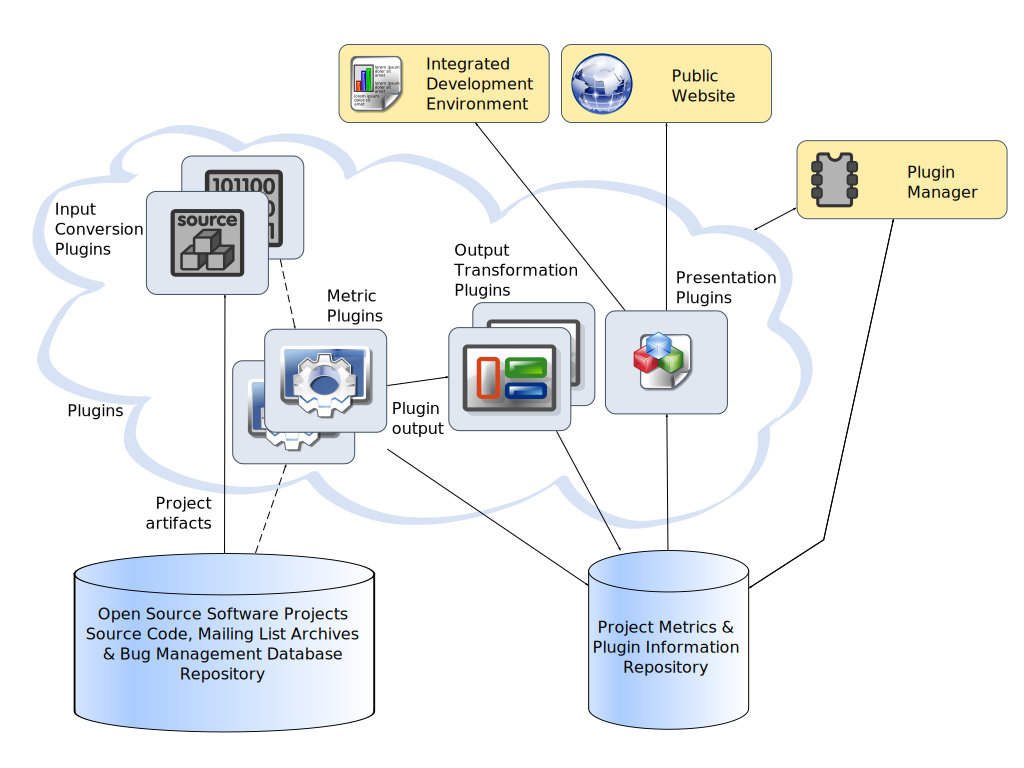
\includegraphics[scale=0.35]{platform-implementation}
	\caption{{\sc sqo-oss} Platform Design}
	\end{center}
\end{figure}

When a new data source (for instance, a new major release of the Linux
kernel) becomes available, the data will be copied on the
{\sc sqo-oss} servers and the system database will be updated
accordingly. All references to the data in {\sc sqo-oss} will be
realised through appropriate queries to the database.  Similarly, when
a new plugin (or a new version of a plugin) becomes available, the
system database will again be updated accordingly. The update process
will be carried out by the plugin manager.

Having both a data source and appropriate plugins, we will be able to
run the plugin on the data source---provided that the plugin is
suitable for the particular data source. In particular, the
\emph{metrics plugins} will be of the following kinds:
\begin{description}
\item [Source code plugins] that calculate a metric directly on source
  code (e.g., count the number of lines of code)
\item [Data mining plugins] that calculate a metric using structured
  and semi-structured information from various parts of a project's
  process data set using data mining techniques
\item [Statistical analysis plugins] that use structured and
  semi-structured information from various parts of a project's process data set
  and the results of other other plugins in order to build statistical
  estimation models that will predict certain events in the project
  development cycle.
\end{description}

Some of the metrics plugins may need the data in a particular format.
The necessary conversion will be the responsibility of \emph{input
  conversion plugins}. For instance, several metrics plugins may
calculate measurements based on a project's configuration management
system logs.
Instead of replicating the functionality of reading and
parsing the logs of configuration management tools like {\sc cvs} and {\sc svn}, the metrics plugins will use
the facilities offered by an appropriate {\sc cvs}-read or {\sc
  svn}-read plugin whose responsibility will be to render the data in
the required format.

After their execution, the metrics plugins will output their results
to the system database. Some plugins may do that directly, but for
some others their output will need to be converted to appropriate
format to be entered in the database, in which case the metrics plugin
output will be chained to suitable \emph{output transformation
  plugins}. To get the results out of the {\sc sqo-oss} database we will 
need \emph{presentation plugins}. These can be a simple matter of 
reading data from the database and returning them as text, or they may 
be converting to {\sc html} or some other required format. These plugins
will be capable of chaining, so that the output of one of them can be
the input of a next one in a transformation sequence.

\subsection{Examples}
\label{subsec:example}

Suppose we want to add a new plugin that will allow us to count the
number of lines of source code. This plugin will be in fact the
Unix {\em wc} utility; in effect we will be teaching {\sc sqo-oss} about
it using the following message:

\begin{verbatim}
<plugin>
  <name>wc</name>
  <version>1</version>
  <applyto>allsrc</applyto>
  <provides>
    <metric>LOC</metric>
  </provides>
  <cmd>xargs cat | wc -l</cmd>
</plugin>
\end{verbatim}

A slightly more involved example, involving the use of the Chidamber
and Kemerer~\cite{CHKE94} object oriented metrics suite for
Java~\cite{SPINELLIS05}, would be:

\begin{verbatim}
<plugin>
  <name>ckjm</name>
  <version>5</version>
  <applyto>javaclasses</applyto>
  <provides>
  	<id>classname</classname>
  	<metric>WMC</metric> <metric>DIT</metric>
  	<metric>NOC</metric> <metric>CBO</metric>
  	<metric>RFC</metric>
  </provides>
  <cmd>java -jar \$JAVALIB/ckjm-1.5.jar</cmd>
</plugin>
\end{verbatim}

In order to call the {\em wc} plugin on a specific target (release 7
of the Free{\sc bsd} operating system) we would send the
following message to {\sc sqo-oss}:

\begin{verbatim}
<plugin>
  <name>wc</name>
  <version>1</version>
  <target>
    <projectid>FreeBSD</projectid>
    <version>RELENG_7</version>
  </target>
</plugin>
\end{verbatim}

In this message, the \texttt{target} refers to a combination of the
project {\sc id} and its version by which a system identifies a given
dataset. The results will be saved as text in the system database.

As explained above, all measurements will be kept into the system
database, so we need a way to retrieve them. To get the output from
the {\em wc} call we would use:

\begin{verbatim}
<transformer>
  <name>text</name>
  <source>measurementid</source>
</transformer>
\end{verbatim}

In the above, the measurement ID could be found by a query such as:

\begin{verbatim}
<query>
  SELECT id FROM Measurement, ProjectVersion, Project
  WHERE ProjectVersionId = ProjectVersion.id
  AND ProjectVersion.ProjectId = Project.id
  AND ProjectVersion.Version = 'RELENG_7'
  AND Project.Name = 'FreeBSD'
</query>
\end{verbatim}

We will be able to chain the output to obtain the desired result:

\begin{verbatim}
<transformer>
  <name>HTML</name>
  <source>
    <transformer>
      <name>text</name>
      <source>measurementid</source>
    </transformer>
  </source>
</transformer>
\end{verbatim}

Similarly, a metric plugin call and output can be combined into a single
call in the obvious way.

The basic interface to the system are messages, like the ones we outlined
above. This allows us to have the same capabilities offered both through a
command line interface and services calls. The plugin descriptors show that
plugins are independent from each other. Hence, plugins for data access are
independent from metrics plugins, so that they can mix and match as
appropriate. Also, we cannot assume that all plugins will be written in the
same language, or that, indeed, we will write all the plugins. The system will
accept any plugin that runs on its operating system platform, as long as it
comes with an acceptable descriptor.

% vbill, gousiosg
% 1000
\section{Expected Results} % {{{1
\label{sec:expected-results}

The software quality observatory for open source software forms a holistic approach to software quality assessment, 
initially targeted towards the specific requirements set by its {\sc oss} 
underpinnings. The three main contributions of the {\sc sqo-oss} project are:
\begin{itemize}
	\item An extensible platform for software quality assessment 
	which can either be used stand-alone or be incorporated into the development 
	process through extensions to popular development tools. The quality 
	assessment plug-ins are fully independent from the main platform. The 
	platform will thus support all programming languages for which there exist 
	quality metric tools.
	\item Combination of readily available metrics with novel techniques 
	involving mining software repositories for project evolution assessment and 
	correlating mailing list information to bug management database entries. Our 
	main scientific contribution can be summarised to the correlation of a large 
	number of product and process metrics with time in an effort to predict 
	future project behavior.
	\item An observatory of quality assessed open source applications. The 
	observatory is going to be updated in an automatic fashion to include the 
	latest versions of the assessed software. The user will also be allowed to 
	customise the observatory results to his/her own needs by means of 
	predefined or custom made quality models	
\end{itemize}

The {\sc sqo-oss} project results will be of interest to a wide number of
audiences. The main target of our focus is on the following categories of users:

\begin{description}
	\item [{\sc it} consultants and {\sc it} managers] Those users need to make 
	informed decisions on software to include into business processes. They are 
	mainly interested in software combining functionality with a proven security 
	record and a predictable future.
The software quality observatory for open source software will enable them 
	to choose among already evaluated software packages and also provide them with 
	the capability to evaluate them in detail according to their needs, as they 
	will have the data and the ability to quantify the quality of a software 
	project.  

	\item [{\sc oss} community] Our aim is to keep
	 open two-way communication channels with the {\sc oss} community. {\sc oss} 
	developers need free tools to assist them with the tedious task of quality 
	assurance. While such tools already exist~\cite{HACK05,SKIB07} they are not 
	open to the community to take advantage of. The {\sc sqo-oss} platform will 
	enable {\sc oss} developers to introduce formal quality control to their 
	projects which will in turn lead to the improved of the community generated 
	software. Furthermore, {\sc sqo-oss} will promote the use of {\sc oss} by 
	providing scientific evidence of its perceived quality.
	
	\item [Researchers] The {\sc sqo-oss} framework can serve as a common testbed 
	for the development of quality evaluation techniques. It will also allow for
	quick prototyping of software quality models by enabling researchers to 
	combine metric results in arbitrary ways.
\end{description}

% all
% 500
\section{Conclusions} % {{{1
\label{sec:conclusions}

The {\sc sqo-oss} system is a platform modeled 
around a pluggable, extensible architecture that enables it to incorporate 
various types of data sources and be accessible through different user interfaces.

Over the past years a new market has been created based on products and value
added services built on top of {\sc f/oss}. In order to allow it to grow, its
products must somehow be comparable to each other, and thus they need to undergo 
some kind of standardization. This is the purpose of a number of research
projects currently funded by the EU, besides {\sc sqo-oss}.
FLOSSMetrics~\cite{FLOS06} stands for Free/Libre/Open Source Software Metrics
and Benchmarking. Its main objective is to construct, publish and analyse a large
scale database with information and metrics about libre software development coming
from several thousands of software projects, using existing methodologies and
tools already developed. {\sc qualoss} stands for {QUAL}ity of Open Source
Software. Its main objective is to provide quality models that will allow
European {\sc sme}s involved in software development to select {\sc f/oss} components
of high quality and integrate them in their systems and products. Quali{PS}o
(Quality Platform for Open Source Software) aims to prepare the industry for
{\sc oss} and vice versa.

{\sc sqo-oss} aims to correlate {\sc OSS} data from various information sources
with the quality characteristics described in Section \ref{sec:quality-attributes}. It
also intends to cooperate with the other related projects, in an attempt to
allow all the involved parties to obtain results faster and combine their
efforts in order to leverage the growth and adoptment of {\sc oss}.

\paragraph*{Acknowledgment} 
This work was partially funded by the European Community's Sixth Framework 
Programme under the contract IST-2005-033331 ``Software Quality Observatory for 
Open Source Software ({\sc sqo-oss})''. 

\bibliographystyle{splncs}
\bibliography{pci07}

\end{document}
